\begin{frame}
\begin{block}{The Algebra of Data Types}
Algebraic Data Types can be thought of in terms of regular algebraic equations
\end{block}
\end{frame}

\begin{frame}
\begin{block}{Some examples include}
\begin{itemize}
  \item<1-> \textbf{sum types}

            \lstinline{Either[A, B]} or ``A or B'' corresponds to the equation \lstinline{A + B}
  \item<2-> \textbf{product types}

            \lstinline{(A, B)} or ``A and B'' corresponds to the equation \lstinline{A * B}
  \item<3-> \textbf{exponentiation}

            \lstinline{A => B} corresponds to the equation \lstinline{B}\textsuperscript{\lstinline{A}}
  \item<4-> \textbf{unit}

            given \lstinline{case class Unit()},

            the \lstinline{Unit} data type corresponds to the value \lstinline{1}
  \item<5-> \textbf{void}

            given \lstinline{private object Void},

            the \lstinline{Void} data type corresponds to the value \lstinline{0}
\end{itemize}
\end{block}
\end{frame}

\begin{frame}[fragile]
\begin{block}{Let's look at \lstinline{Bool}}
\begin{lstlisting}[style=scala]
sealed trait Bool
case class True() extends Bool
case class False() extends Bool
\end{lstlisting}
\begin{itemize}
  \item<1-> The \lstinline{True} constructor has no arguments, which is equivalent to carrying \lstinline{Unit}
  \item<1-> The \lstinline{False} constructor has no arguments, which is equivalent to carrying \lstinline{Unit}
  \item<2-> The whole data type carries \lstinline{1} or \lstinline{1}
  \item<2-> \lstinline{Bool ~ 1 + 1 ~ 2}
\end{itemize}
\end{block}
\end{frame}

\begin{frame}[fragile]
\begin{block}{How about \lstinline{Option[A]}}
\begin{lstlisting}[style=scala]
sealed trait Option[A]
case class None[A]() extends Option[A]
case class Some[A](a: A) extends Option[A]
\end{lstlisting}
\begin{itemize}
  \item<1-> The \lstinline{None} constructor has no arguments, which is equivalent to carrying \lstinline{Unit}
  \item<1-> The \lstinline{Some} constructor has an argument \lstinline{A}
  \item<2-> The whole data type carries \lstinline{1} or \lstinline{A}
  \item<2-> \lstinline{Option[A] ~ 1 + A}
\end{itemize}
\end{block}
\end{frame}

\begin{frame}[fragile]
\begin{block}{Another one \lstinline{Either[Void, A]}}
\begin{lstlisting}
\end{lstlisting}
\begin{itemize}
  \item<1-> The \lstinline{Left} constructor carries \lstinline{0}
  \item<1-> The \lstinline{Right} constructor has an argument \lstinline{A}
  \item<2-> The whole data type carries \lstinline{0} or \lstinline{A}
  \item<2-> \lstinline{Either[Void, A] ~ 0 + A ~ A}
\end{itemize}
\end{block}
\end{frame}

\begin{frame}[fragile]
\begin{block}{and another \lstinline{(Void, A)}}
\begin{lstlisting}
\end{lstlisting}
\begin{itemize}
  \item<1-> The whole data type carries \lstinline{0} and \lstinline{A}
  \item<2-> \lstinline{(Void, A) ~ 0 * A ~ 0}
\end{itemize}
\end{block}
\end{frame}

\begin{frame}
\begin{block}{lots of \lstinline{Bool}}
\begin{itemize}
  \item<1-> \lstinline{(Bool, Bool)}
  \item<1-> \lstinline{Either[Bool, Bool]}
  \item<1-> \lstinline{Bool => Bool}
  \item<2-> \lstinline{2 * 2}
  \item<2-> \lstinline{2 + 2}
  \item<2-> \lstinline{2}\textsuperscript{\lstinline{2}}
  \item<3-> These are all \lstinline{4}
\end{itemize}
\end{block}
\end{frame}

\begin{frame}
\begin{block}{Inhabitants}
The resulting algebraic equation gives us the number of \emph{inhabitants}.

Or, the number of values with that type.
\end{block}
\end{frame}

\begin{frame}
\begin{block}{Inhabitants}
\begin{itemize}
  \item<1-> \lstinline{Option[Bool => Maybe Bool]}
  \item<1-> has \lstinline{1 + (1 + 2)}\textsuperscript{\lstinline{2}} inhabitants
  \item<1-> \lstinline{9} inhabitants
  \item<2-> \tiny{\lstinline{(Either[Bool, Option[Bool]], Bool, (Unit, Bool), Either[Void, Bool])}}
  \item<2-> has \lstinline{(2 + (1 + 2)) * 2 * (1 * 2) * (0 + 2)} inhabitants
  \item<2-> \lstinline{40}
\end{itemize}
\end{block}
\end{frame}

\begin{frame}
\begin{block}{Algebraically}
\begin{center}
What is \lstinline{List[A]}?
\end{center}
\end{block}
\end{frame}

\begin{frame}
\begin{block}{Lists}
\begin{itemize}
  \item<1-> \lstinline{List[A]} is either zero \lstinline{A} or one \lstinline{A} or two \lstinline{A} \ldots
  \item<2-> \lstinline{A}\textsuperscript{\lstinline{0}} \lstinline{+ A}\textsuperscript{\lstinline{1}} \lstinline{+ A}\textsuperscript{\lstinline{2}} \ldots
  \item<3-> using algebraic rules, this simplifies to \lstinline{1 + A * List[A]}
  \item<3-> \lstinline{1} or \lstinline{(A and List[A])}
  \item<3-> The \lstinline{Nil} \emph{(carrying \lstinline{Unit})} or \lstinline{(::)} constructor
\end{itemize}
\end{block}
\end{frame}


\begin{frame}
\begin{center}
Let's \textbf{really} emphasise the algebra of data types
\end{center}
\end{frame}

\begin{frame}
\begin{center}
Remember calculus?
\end{center}
\end{frame}


\begin{frame}
\begin{center}
Me neither :)
\end{center}
\end{frame}


\begin{frame}
\begin{center}
Here is a data type:

\lstinline{Either[X, (X, X)]}
\end{center}
\end{frame}


\begin{frame}
\begin{center}
Algebraically:

\lstinline{X + (X * X)}
\end{center}
\end{frame}


\begin{frame}
\begin{center}
Differentiate

$\frac{\partial}{\partial X}$ \lstinline{(X + (X * X))}
\end{center}
\end{frame}


\begin{frame}
\begin{center}
$\frac{\partial}{\partial X}$ \lstinline{(X + (X * X))}

\tiny{\emph{(sum rule)}}\normalsize{}

\lstinline{=} $\frac{\partial}{\partial X}$ \lstinline{(X +} $\frac{\partial}{\partial x}$ \lstinline{(X * X))}

\tiny{\emph{(power rule, line rule)}}\normalsize{}

\lstinline{= 1 + (2 * X)}

\par\noindent\rule{\textwidth}{0.4pt}

\lstinline{= Option[(Bool, X)]}
\end{center}
\end{frame}


\begin{frame}
\begin{block}{$\therefore$}
\begin{center}
$\frac{\partial}{\partial X}$ \lstinline{Either[X, (X, X)]}

\par\noindent\rule{\textwidth}{0.4pt}

\lstinline{= Option[(Bool, X)]}
\end{center}
\end{block}
\end{frame}


\begin{frame}
\begin{center}
We'll do another one

\lstinline{(Either[X, X], Either[X, X])}
\end{center}
\end{frame}


\begin{frame}
\begin{center}
Algebraically:

\lstinline{(X + X) * (X + X)}
\end{center}
\end{frame}


\begin{frame}
\begin{center}
Differentiate

$\frac{\partial}{\partial X}$ \lstinline{((X + X) * (X + X))}
\end{center}
\end{frame}


\begin{frame}
\begin{center}
$\frac{\partial}{\partial X}$ \lstinline{((X + X) * (X + X))}

\lstinline{=} $\frac{\partial}{\partial X}$ \lstinline{4 * X}\textsuperscript{\lstinline{2}}

\tiny{\emph{(power rule)}}\normalsize{}

\lstinline{= 4 *} $\frac{\partial}{\partial X}$ \lstinline{X}\textsuperscript{\lstinline{2}}

\tiny{\emph{(power rule)}}\normalsize{}

\lstinline{= 4 * 2 * X}

\par\noindent\rule{\textwidth}{0.4pt}

\lstinline{= 8 * X}
\end{center}
\end{frame}


\begin{frame}
\begin{block}{$\therefore$}
\begin{center}
$\frac{\partial}{\partial X}$ \lstinline{(Either[X, X], Either[X, X])}

\par\noindent\rule{\textwidth}{0.4pt}

\lstinline{= (Option[Bool] => Bool, X)}
\end{center}
\end{block}
\end{frame}


\begin{frame}
\begin{center}
A simpler one

\lstinline{(X, X, X)}
\end{center}
\end{frame}


\begin{frame}
\begin{center}
Algebraically:

\lstinline{X * X * X}
\end{center}
\end{frame}


\begin{frame}
\begin{center}
Differentiate

$\frac{\partial}{\partial X}$ \lstinline{X * X * X}
\end{center}
\end{frame}


\begin{frame}
\begin{center}
$\frac{\partial}{\partial X}$ \lstinline{X * X * X}

\lstinline{=} $\frac{\partial}{\partial X}$ \lstinline{X}\textsuperscript{\lstinline{3}}

\tiny{\emph{(power rule)}}\normalsize{}

\lstinline{= 3 *} \lstinline{X}\textsuperscript{\lstinline{2}}
\end{center}
\end{frame}


\begin{frame}
\begin{block}{$\therefore$}
\begin{center}
$\frac{\partial}{\partial X}$ \lstinline{(X, X, X)}

\par\noindent\rule{\textwidth}{0.4pt}

\lstinline{= (Maybe Bool, X, X)}
\end{center}
\end{block}
\end{frame}


\begin{frame}
\begin{center}
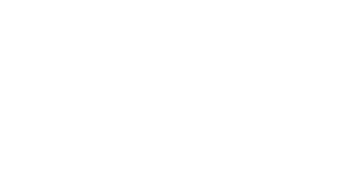
\includegraphics[width=0.3\textheight]{image/crosseyed-blank.png}
\end{center}
\begin{block}{Summary}
\begin{itemize}
  \item \scriptsize{$\frac{\partial}{\partial X}$ \lstinline{Either[X, (X, X)] = Option[(Bool, X)]}}
  \item \scriptsize{$\frac{\partial}{\partial X}$ \lstinline{(Either[X, X], Either[X, X]) = (Option[Bool => Bool], X)}}
  \item \scriptsize{$\frac{\partial}{\partial X}$ \lstinline{(X, X, X) = (Option[Bool], X, X)}}
\end{itemize}
\end{block}
\end{frame}

\begin{frame}
\begin{block}{Let's do list}
\lstinline{List[A] = 1 + A + A}\textsuperscript{\lstinline{2}} \lstinline{+ A}\textsuperscript{\lstinline{3}} \lstinline{+} \ldots
\end{block}
\end{frame}

\begin{frame}{List}

\lstinline{List[A] = 1 + A + A}\textsuperscript{\lstinline{2}} \lstinline{+ A}\textsuperscript{\lstinline{3}} \lstinline{+} \ldots

\par\noindent\rule{\textwidth}{0.4pt}

\lstinline{let K A = A + A}\textsuperscript{\lstinline{2}} \lstinline{+ A}\textsuperscript{\lstinline{3}} \lstinline{+} \ldots

\lstinline{List A = 1 + K A}

\emph{\tiny{multiply list by \lstinline{A}}}

\lstinline{K A = A * List[A]}

\par\noindent\rule{\textwidth}{0.4pt}

{$\therefore$} List[A] = 1 + A * List[A]

\emph{\tiny{this makes sense if we think of \lstinline{List} in terms of its constructors}}

\end{frame}


\begin{frame}{List}

\lstinline{List[A] = 1 + A * List[A]}

\par\noindent\rule{\textwidth}{0.4pt}

\emph{\tiny{subtract \lstinline{(A * List[A])} both sides}}

\lstinline{List[A] - (A * List[A]) = 1}

\emph{\tiny{multiply \lstinline{List[A]} by \lstinline{1}}}

\lstinline{(1 * List[A]) - (A * List[A]) = 1}

\emph{\tiny{apply distributive law of multiplication}}

\lstinline{List[A] * (1 - A) = 1}

\emph{\tiny{divide both sides by \lstinline{1 - A}}}

\lstinline{List[A] = 1 / (1 - A)}

\par\noindent\rule{\textwidth}{0.4pt}

\emph{\tiny{apply exponent rule}}

{$\therefore$} \lstinline{List[A] = (1 - A)}\textsuperscript{\lstinline{-1}}

\end{frame}


\begin{frame}{List}

\lstinline{List[A] = (1 - A)}\textsuperscript{\lstinline{-1}}

\par\noindent\rule{\textwidth}{0.4pt}

\lstinline{let u = 1 - A}

\emph{\tiny{apply chain rule}}

$\frac{\partial}{\partial a}$ {\lstinline{(1 - A)}\textsuperscript{\lstinline{-1}}} \lstinline{=} $\frac{\partial}{\partial u}$ {\lstinline{u}\textsuperscript{\lstinline{-1}}} \lstinline{*} $\frac{\partial}{\partial A}$ \lstinline{1 - A}

\emph{\tiny{differentiate \lstinline{u}\textsuperscript{\lstinline{-1}}}}

$\frac{\partial}{\partial u}$ \lstinline{u}\textsuperscript{\lstinline{-1}} \lstinline{=} \lstinline{-1 / u}\textsuperscript{\lstinline{2}}

\emph{\tiny{differentiate \lstinline{1 - A}}}

$\frac{\partial}{\partial A}$ \lstinline{1 - A} \lstinline{= -1} 

\par\noindent\rule{\textwidth}{0.4pt}

{$\therefore$} $\frac{\partial}{\partial A}$ {\lstinline{(1 - A)}\textsuperscript{\lstinline{-1}}} \lstinline{=} \lstinline{(-1 / u}\textsuperscript{\lstinline{2}}\lstinline{) * -1}

\end{frame}


\begin{frame}{List}

$\frac{\partial}{\partial A}$ {\lstinline{(1 - A)}\textsuperscript{\lstinline{-1}}} \lstinline{=} \lstinline{(-1 / u}\textsuperscript{\lstinline{2}}\lstinline{) * -1}

\par\noindent\rule{\textwidth}{0.4pt}

\emph{\tiny{substitute back \lstinline{u = 1 - A}}}

$\frac{\partial}{\partial A}$ {\lstinline{(1 - A)}\textsuperscript{\lstinline{-1}}} \lstinline{=} \lstinline{(-1 / (1 - A)}\textsuperscript{\lstinline{2}}\lstinline{) * -1}

\emph{\tiny{simplify by multiplying right side by \lstinline{-1}}}

$\frac{\partial}{\partial A}$ {\lstinline{(1 - A)}\textsuperscript{\lstinline{-1}}} \lstinline{=} \lstinline{1 / (1 - A)}\textsuperscript{\lstinline{2}}

\emph{\tiny{apply exponent rule}}

$\frac{\partial}{\partial A}$ {\lstinline{(1 - A)}\textsuperscript{\lstinline{-1}}} \lstinline{=} \lstinline{(1 / 1 - A)}\textsuperscript{\lstinline{2}}

$\frac{\partial}{\partial A}$ {\lstinline{(1 - A)}\textsuperscript{\lstinline{-1}}} \lstinline{=} \lstinline{((1 - A)}\textsuperscript{\lstinline{-1}}\lstinline{)}\textsuperscript{\lstinline{2}}

\par\noindent\rule{\textwidth}{0.4pt}

{$\therefore$} The derivative of a \lstinline{List} is a pair of \lstinline{List}

\end{frame}

\begin{frame}
\begin{block}{The whole point of this exercise \ldots}
is to encourage thinking \emph{algebraically} about our data types
\end{block}
\end{frame}

\begin{frame}[fragile]
\begin{block}{including this one \ldots}
\begin{lstlisting}[style=scala]
trait BlahService[F[_]] {
  def validateBlib(img: Stream[F, Byte]):
    F[Either[Error, Unit]]
  def validateBlob(img: Stream[F, Byte]):
    F[Either[Error, Unit]]
  def calculateBlab(img: Stream[F, Byte]):
    F[Either[Error, Blab]]
}
\end{lstlisting}
\end{block}
\end{frame}

\begin{frame}
\begin{center}
\ldots and others like it
\end{center}
\end{frame}
